\chapter{Commonly Used Terms}
\begin{description}
	\item[Blockchain] A shared, immutable ledger for recording the history of transactions in blocks.
	\item[Block] A defined data structure that contains a record of transaction data and other values.
	\item[XSPEC] The symbol (ticker) for Spectrecoin and also the name of the public coins on the blockchain.
	\item[SPECTRE] The name used for the private coins on the Spectrecoin blockchain.
	\item[UTXO] Unspent Transaction Output that can be spent as an input in a new transaction.
	\item[ATXO] UTXO that can be spent as in input in a private transaction using a ring signature.
	\item[Keyimage] A unique value associated with a specific ATXO calculated using a private key.
	\item[Spent (UTXO)] A UTXO is spent when it has been ‘consumed’ as an input in a new transaction.
	\item[Spent (ATXO)] An ATXO is spent when the related ‘keyimage’ has been included in a valid ring signature.
	\item[Hash function] A mathematical one-way function that generates fixed size data from an arbitrary input.
	\item[Hash value] A numeric \textbf{value} of a fixed length that uniquely identifies the data input in a hash function.
	\item[Block hash] The hash of a block's header.
	\item[Kernel Hash] A hash value used in Proof-of-Stake.
	\item[Mixin] A chaff or dummy ATXO not being spent in a current transaction, used in a ring signature.
	\item[TOR] The Onion Router. A layered network that attempts to hide your IP address.
	\item[VIN] The ‘collection’ of input data for a transaction, including the UTXOs/ATXOs to be consumed.
	\item[VOUT] The ‘collection’ of output data for a transaction, including the new UTXOs/ATXOs generated.
	\item[PoS] Proof-of-Stake. A consensus mechanism introduced with Peercoin
	\item[PoSv3] Proof-of-Stake v3. Consensus mechanism developed by the Blackcoin developers.
	\item[PoAS] Proof-of-Anonymous-Stake. Privacy consensus mechanism introduced by the Spectrecoin developers.
\end{description}



We will use some screenshots from the Spectrecoin block explorer
\footnote{https://chainz.cryptoid.info/xspec/} to show examples of
transactions and to explain some of the features. The block explorer
is not custom made for Spectrecoin and will always show ‘\textit{XSPEC}’
as the designation behind a value. When this is preceded by the word
‘\textit{Anonymous}’ it designates a SPECTRE value.

\begin{figure}[h]
	\caption{Example of a parametric plot ($\sin (x), \cos(x), x$)}
	\centering
	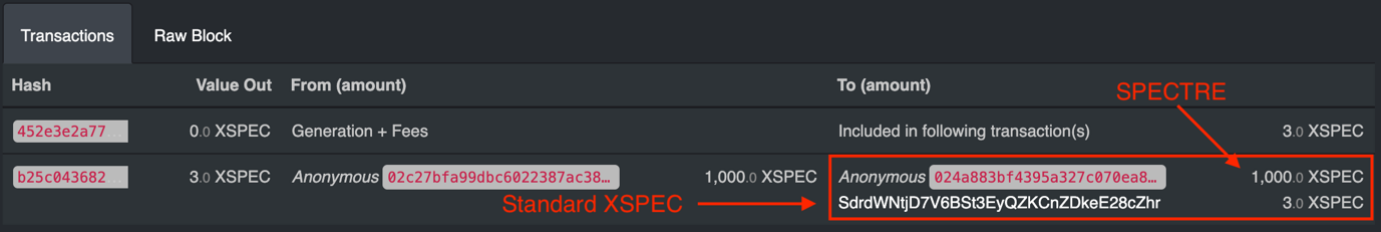
\includegraphics[width=\textwidth]{ExampleStakingTransaction.png}
\end{figure}


References are designated by superscript (numbers) and relate to the relevant
footnotes and links at the bottom of each page. Please follow the links to
explore certain topics in more detail.
